\begin{flushright} {\tiny {\color{gray} benchmark\_stokes\_sphere\_fs\_2D.tex}} \end{flushright}

The domain is a $1\times 0.75$ box. If sticky air is used, then its thickness should be 0.25 so that the
domain is a unit square. 
The fluid is characterised by $\rho_f=1$ and $\eta_f=1$. The sphere is characterised by $\rho_s=2$ and
$\eta_s=10^3$. The air is characterised by $\rho_a=0$ and $\eta_a=10^{-3}$. Gravity is 
vertical with $\vec{g}=-\vec{e}_y$.
The sphere has a radius $R_S=0.123456789$ and its center is at position $\vec{r}_c=(0.5,0.6)$. 
Boundary conditions are free slip on all sides (unless a true free surface is used).
Pressure is normalised so that its average is zero on the top (if no free surface is used).
The model is run for 200s. The CFL number is set to 0.25 with a maximum time step of 0.5. 

We wish to keep track of the following quantities as a function of time:
\begin{itemize}
\item the position and velocity of the sphere center,
\item the minimum and maximum topography,
\item the volume of fluid $V_f(t)$, sphere $V_s(t)$ and air $V_a(t)$
\item root mean square velocity $\upnu_{vrms}$ for the whole domain, as well as for the air, fluid and sphere 
      separately, and for the fluid+sphere,
\item the maximum velocity and pressure in the domain,
\item the time step value $\delta t$,
\item the average density\footnote{Because $L_xL_y=1$, also equal to the total mass of the system} and viscosity in the domain:
\begin{eqnarray}
\langle \rho \rangle (t) &=& \frac{1}{L_xL_y} \iint \rho(x,y,t) dx dy
= \frac{1}{L_xL_y} ( V_a(t)\rho_a + V_f(t)\rho_f + V_s(t)\rho_s )  \nn\\
\langle \eta \rangle (t) &=& \frac{1}{L_xL_y} \iint \eta(x,y,t) dx dy
\frac{1}{L_xL_y} ( V_a(t) \eta_a + V_f(t)\eta_f  + V_s(t)\eta_s ) 
\end{eqnarray}
Initial values are 
\[
\langle \rho \rangle (0) = \frac{1}{L_xL_y} ( V_a(0)\rho_a + V_f(0)\rho_f + V_s(0)\rho_s )  
= 0.25*0 + (0.75-\pi R_s^2)*1 + \pi R_s^2* 2 = 0.75 + \pi R_s^2  \simeq 0.79788283183
\]
\[
\langle \eta \rangle (0) = \frac{1}{L_xL_y} ( V_a(0)\eta_a + V_f(0)\eta_f + V_s(0)\eta_s )  
= 0.25*10^{-3} + (0.75-\pi R_s^2)*1 + \pi R_s^2* 10^3   \simeq 48.5851989989
\]



\item the min/max of the compositional fields when these are used;
\item the velocity, pressure and material at position (0.5,0.6);
\item the pressure at position (0.5,0).
\end{itemize}

Participating codes:
\begin{itemize}
\item \aspect{} uses $Q_2\times Q_1$ elements by default. $Q_2\times P_{-1}$
elements can be used by setting
\begin{lstlisting}
subsection Discretization
  set Use locally conservative discretization = true
end
\end{lstlisting}
The default stabilisation method when compositional fields are used is the 
entropy viscosity method, but SUPG has also been implemented and can be 
triggered with 
\begin{lstlisting}
subsection Discretization
  subsection Stabilization parameters
    set Stabilization method = SUPG
  end
end
\end{lstlisting}

The default mesh settings are as follows:
\begin{lstlisting}
subsection Mesh refinement
  set Initial adaptive refinement   = 1 
  set Initial global refinement     = 6 
  set Refinement fraction           = 0.9 
  set Strategy                      = composition
  set Coarsening fraction           = 0.1 
end
\end{lstlisting}

In the results hereafter when the combination 6-0 or 7-0 are mentioned, this means that the coarsening 
fraction has been set to zero and these correspond then to regular meshes with 64x64 and 128x128 elements
respectively.

Active particles can also replace the compositional fields and this is how it is triggered from the input file:

\begin{lstlisting}
subsection Compositional fields
  set Number of fields = 2 
  set Names of fields = sphere, air 
  set Compositional field methods = particles, particles
  set Mapped particle properties = sphere:initial sphere, air: initial air 
end

subsection Postprocess
  set List of postprocessors = visualization, ... , particles
  subsection Visualization
    set List of output variables = density, viscosity, strain rate
    set Time between graphical output = 1 
  end 
  subsection Particles
    set Number of particles = 100000
    set Time between data output = 0 
    set Data output format = vtu 
    set List of particle properties = velocity, initial composition, initial position #, integrated strain
    set Interpolation scheme = cell average
    set Update ghost particles = true
    set Particle generator name = random uniform
  end 
end
\end{lstlisting}

 

 
\item Stone 93. Code based on unstructured mesh of Crouzeix-Raviart triangular elements.
 The resolution is controlled by the minimum area of 
the triangles as passed as argument to the triangle mesher, and the parameter $np$ which controls
the number of points on the hull ($np$ on each side), the surface ($5*np$) and the sphere ($5*np$);

\item Alessandro Regorda's code:
The number of markers is fixed per element with random distribution.
At the beginning of the simulation there are: 562500 for 150x150 grid with 25 markers per element, 
600,000 for 200x200 grid with 15 markers per element,
655,360 for 256x256 grid with 10 markers per element,
2,621,440 for 512x512 grid with 10 markers per element.

The advection is RK4. The code maintains the number of markers per element between half of the
initial number and the initial number plus half (e.g. in 512x512
markers are between 5 and 15). When in an element there are less
markers than the minimum it adds random markers to reach the minimum,
while if the number is higher than the maximum some of them are
deleted. In this way elements are never empty. When new markers are
added they assume the type of the nearest marker.
Averaging only applies to viscosity, density is always arithmetically
averaged.




\end{itemize}

In what follows 6-0 and 7-0 correspond to regular grids (no coarsening, no refinement) 

\newpage
\paragraph{Root mean square velocity}

\begin{center}
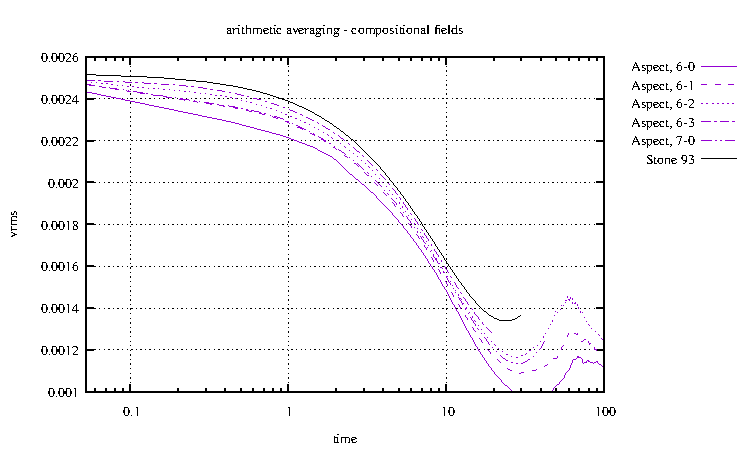
\includegraphics[width=5.7cm]{images/stokes_sphere_fs2D/vrms_arithm_comp}
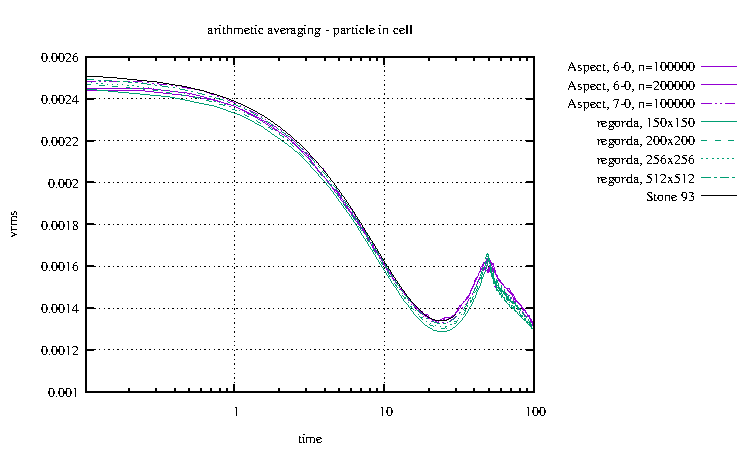
\includegraphics[width=5.7cm]{images/stokes_sphere_fs2D/vrms_arithm_pic}
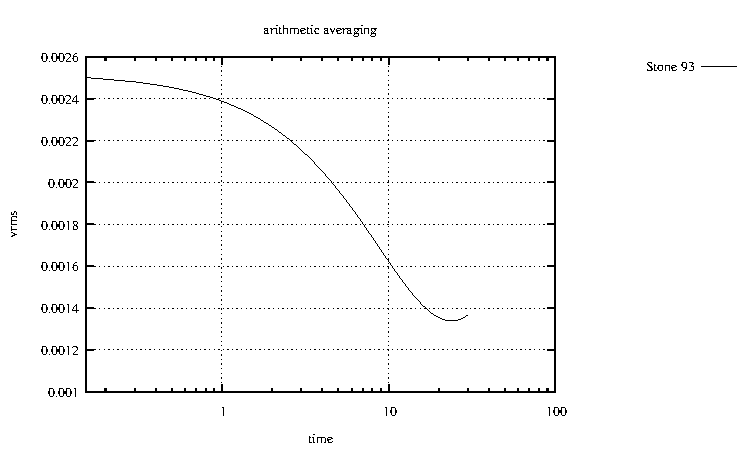
\includegraphics[width=5.7cm]{images/stokes_sphere_fs2D/vrms_arithm_add}\\
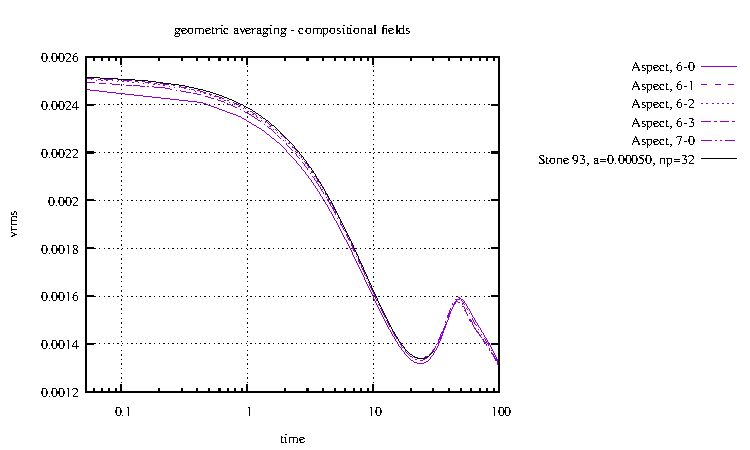
\includegraphics[width=5.7cm]{images/stokes_sphere_fs2D/vrms_geom_comp}
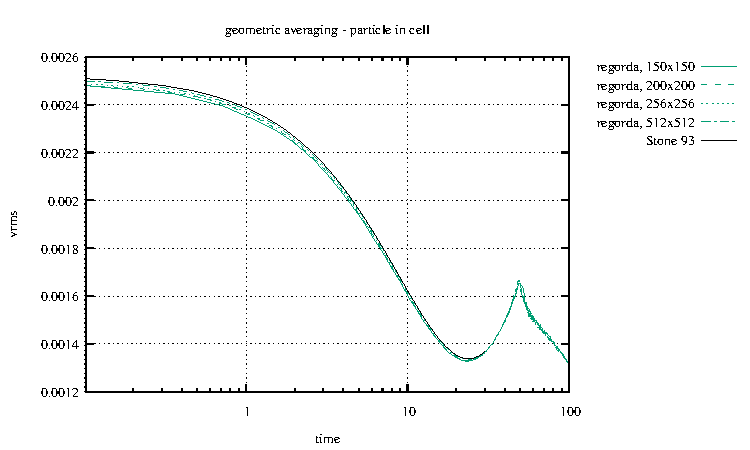
\includegraphics[width=5.7cm]{images/stokes_sphere_fs2D/vrms_geom_pic}
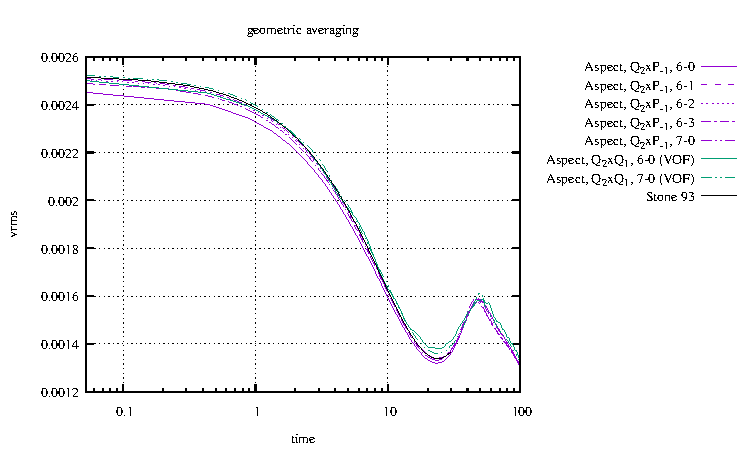
\includegraphics[width=5.7cm]{images/stokes_sphere_fs2D/vrms_geom_add}\\
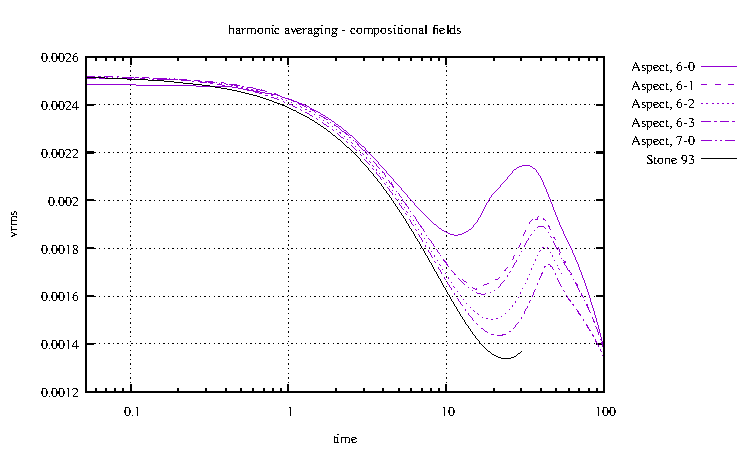
\includegraphics[width=5.7cm]{images/stokes_sphere_fs2D/vrms_harm_comp}
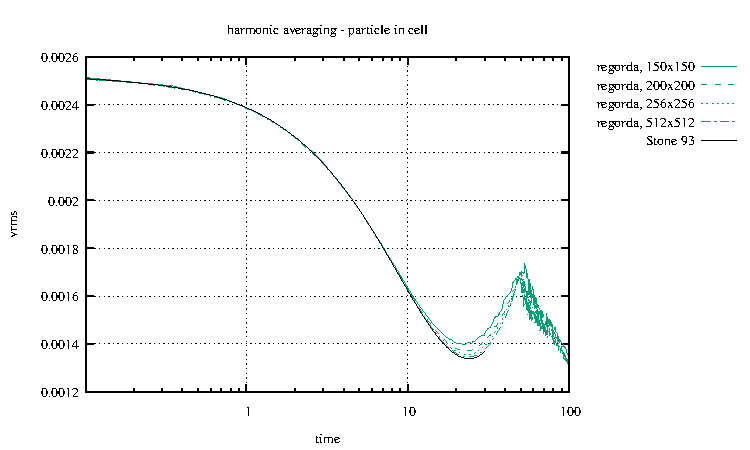
\includegraphics[width=5.7cm]{images/stokes_sphere_fs2D/vrms_harm_pic}
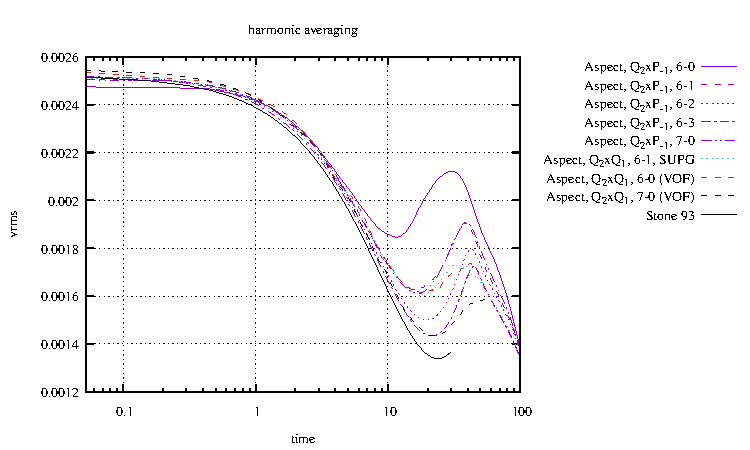
\includegraphics[width=5.7cm]{images/stokes_sphere_fs2D/vrms_harm_add}\\
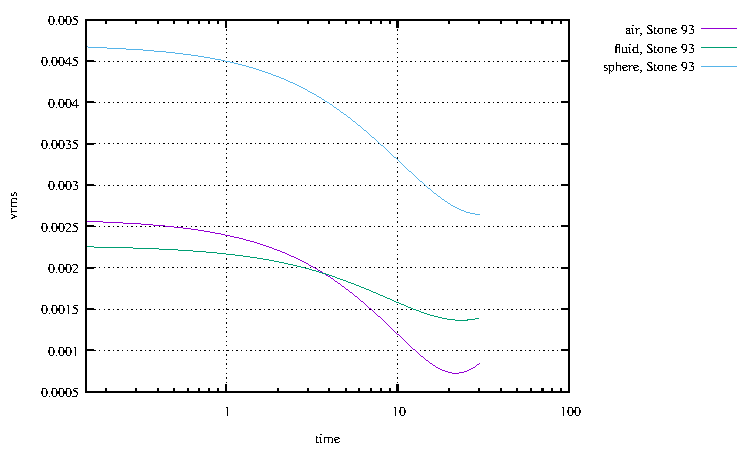
\includegraphics[width=5.7cm]{images/stokes_sphere_fs2D/vrms_afs}
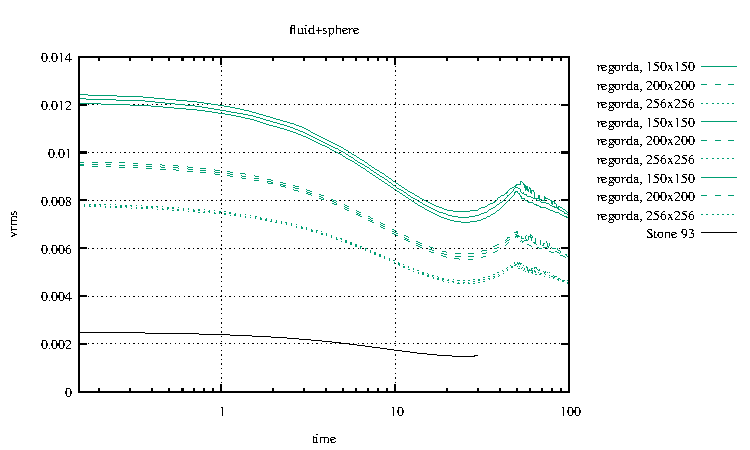
\includegraphics[width=5.7cm]{images/stokes_sphere_fs2D/vrms_fs}
\end{center}

\paragraph{Volumes}
\begin{center}
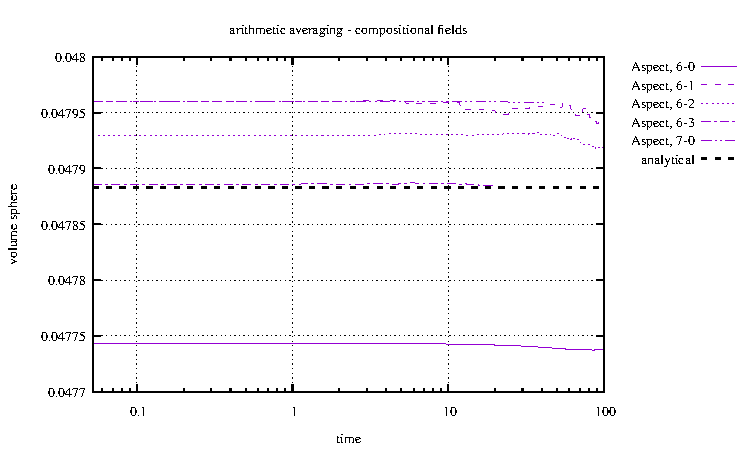
\includegraphics[width=5.7cm]{images/stokes_sphere_fs2D/vol_sphere_arithm_comp}
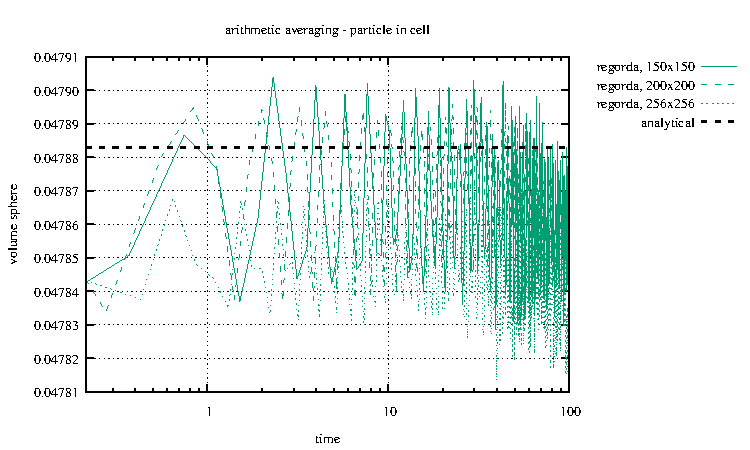
\includegraphics[width=5.7cm]{images/stokes_sphere_fs2D/vol_sphere_arithm_pic}
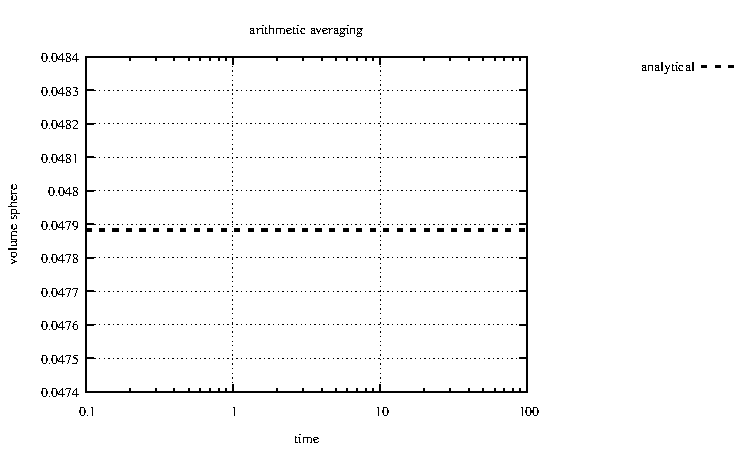
\includegraphics[width=5.7cm]{images/stokes_sphere_fs2D/vol_sphere_arithm_add}\\
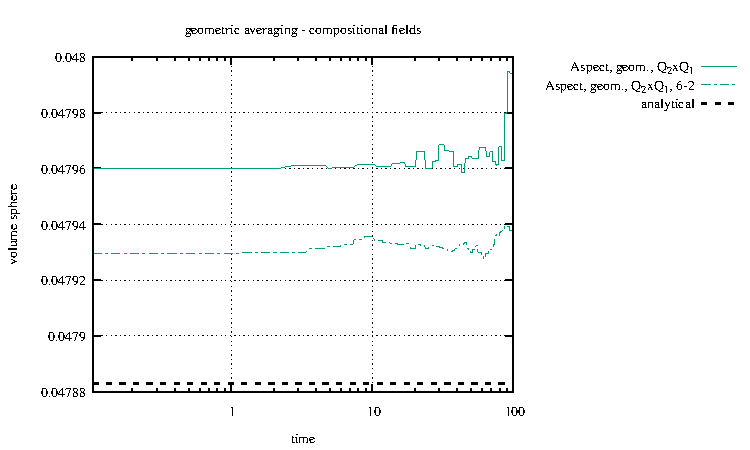
\includegraphics[width=5.7cm]{images/stokes_sphere_fs2D/vol_sphere_geom_comp}
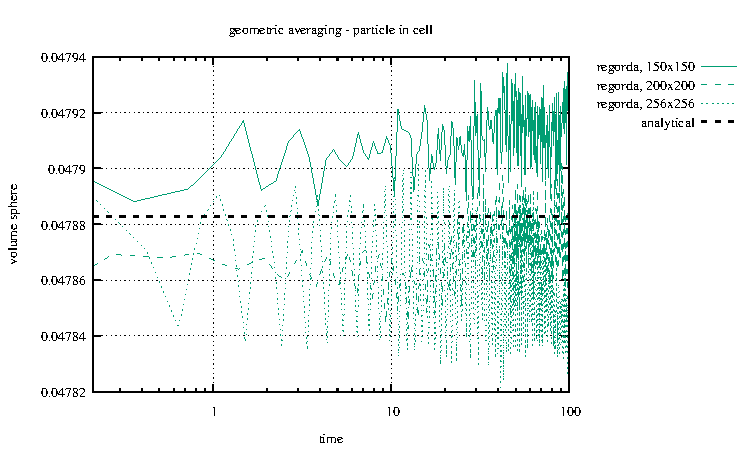
\includegraphics[width=5.7cm]{images/stokes_sphere_fs2D/vol_sphere_geom_pic}
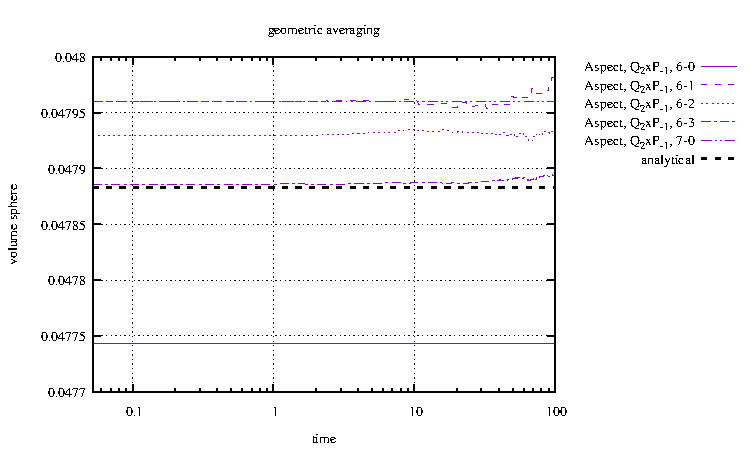
\includegraphics[width=5.7cm]{images/stokes_sphere_fs2D/vol_sphere_geom_add}\\
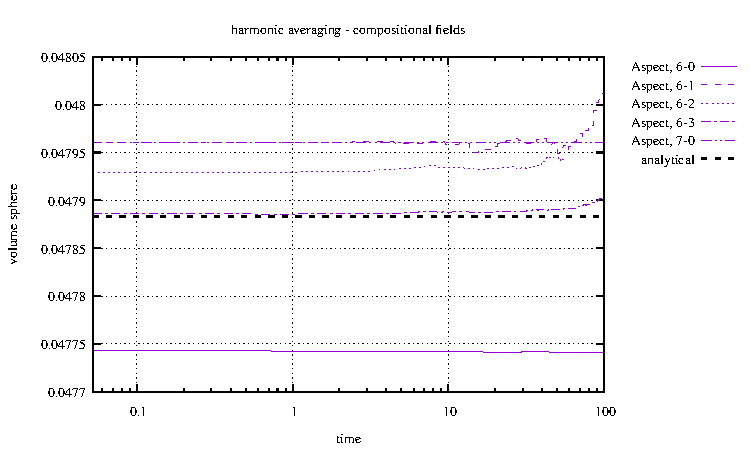
\includegraphics[width=5.7cm]{images/stokes_sphere_fs2D/vol_sphere_harm_comp}
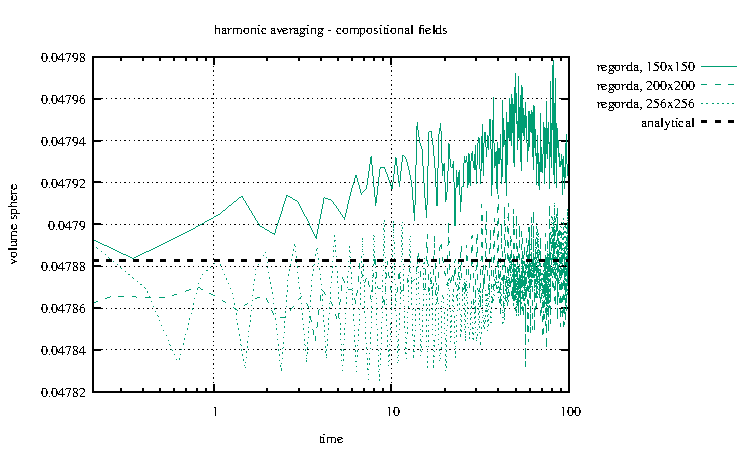
\includegraphics[width=5.7cm]{images/stokes_sphere_fs2D/vol_sphere_harm_pic}
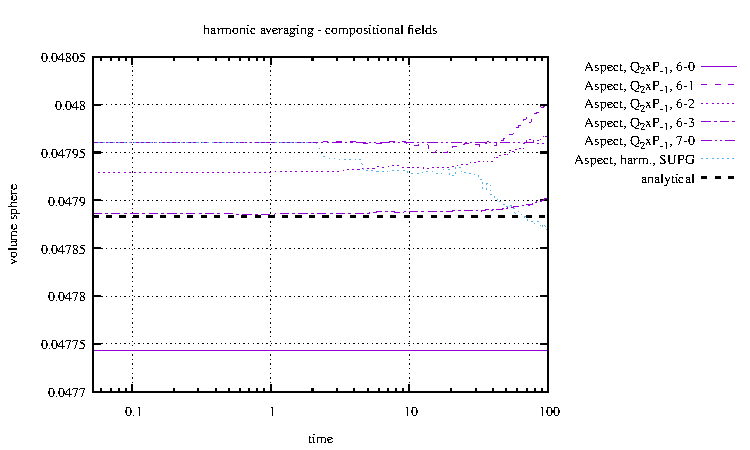
\includegraphics[width=5.7cm]{images/stokes_sphere_fs2D/vol_sphere_harm_add}
%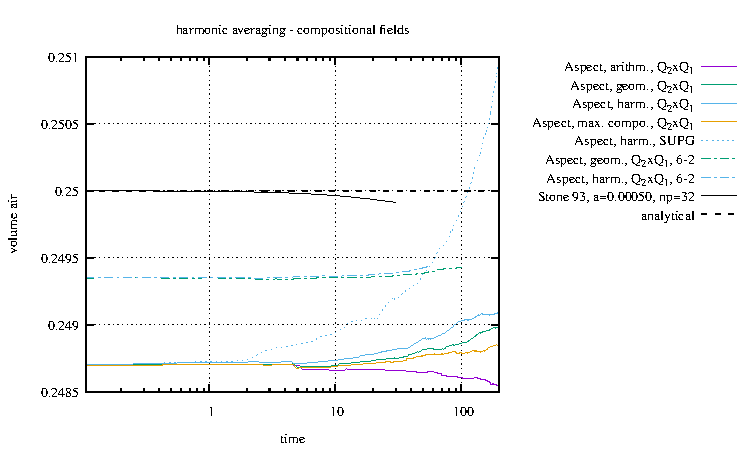
\includegraphics[width=7cm]{images/stokes_sphere_fs2D/vol_air} 
%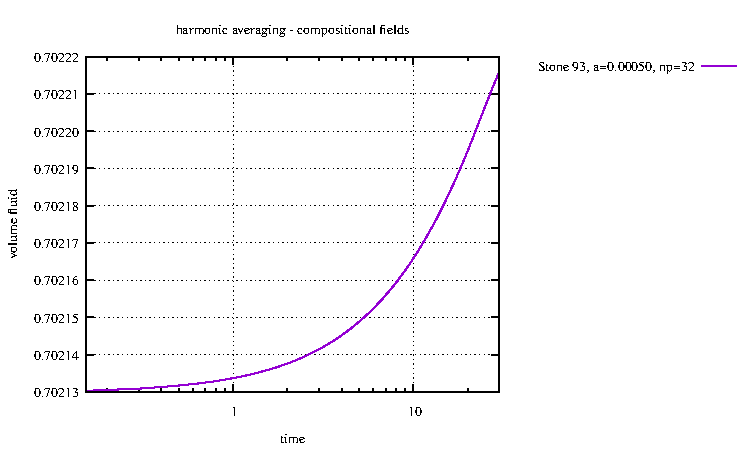
\includegraphics[width=7cm]{images/stokes_sphere_fs2D/vol_fluid}\\
%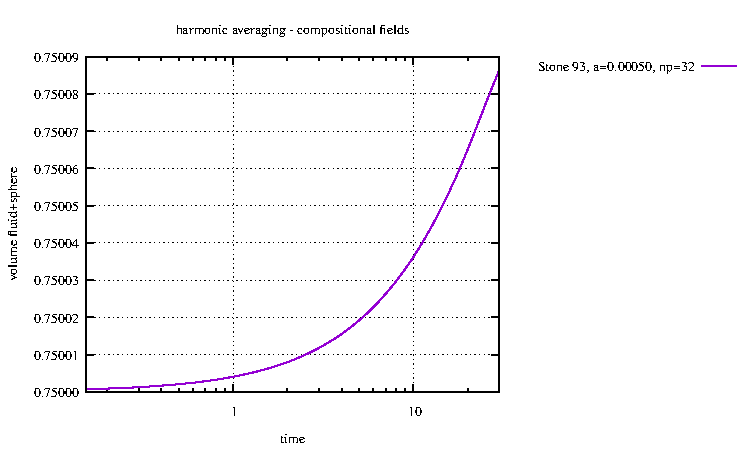
\includegraphics[width=7cm]{images/stokes_sphere_fs2D/vol_fluidsphere}
\end{center}


\paragraph{Maximum velocity}
\begin{center}
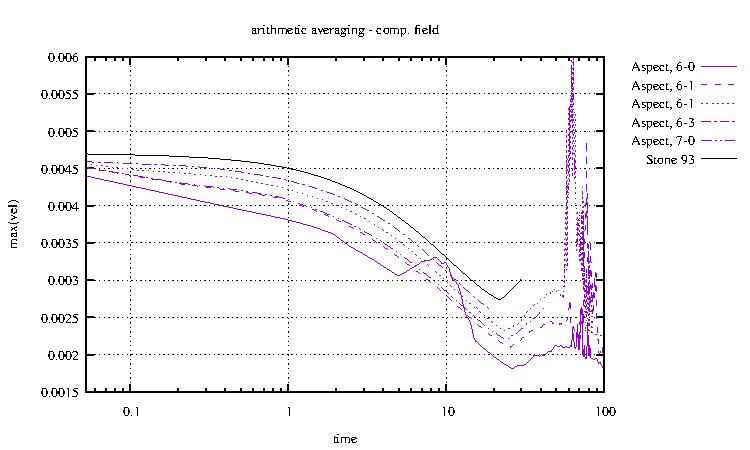
\includegraphics[width=5.7cm]{images/stokes_sphere_fs2D/max_vel_arithm_comp}
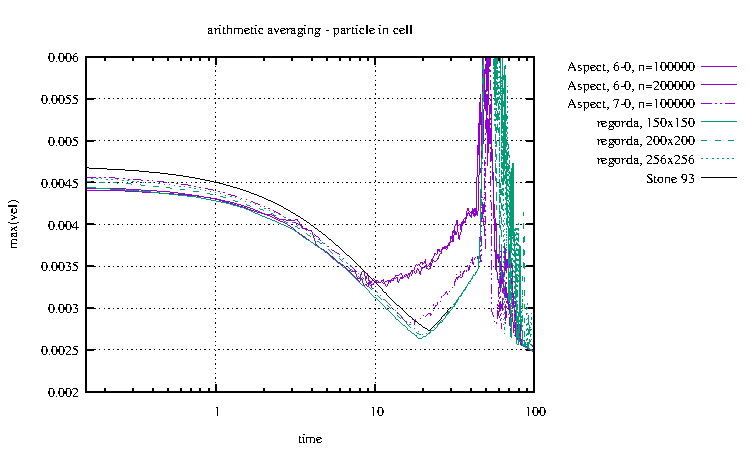
\includegraphics[width=5.7cm]{images/stokes_sphere_fs2D/max_vel_arithm_pic}
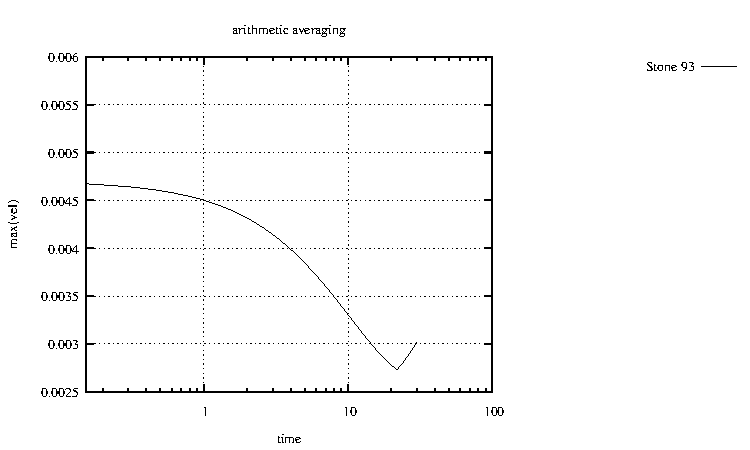
\includegraphics[width=5.7cm]{images/stokes_sphere_fs2D/max_vel_arithm_add}\\
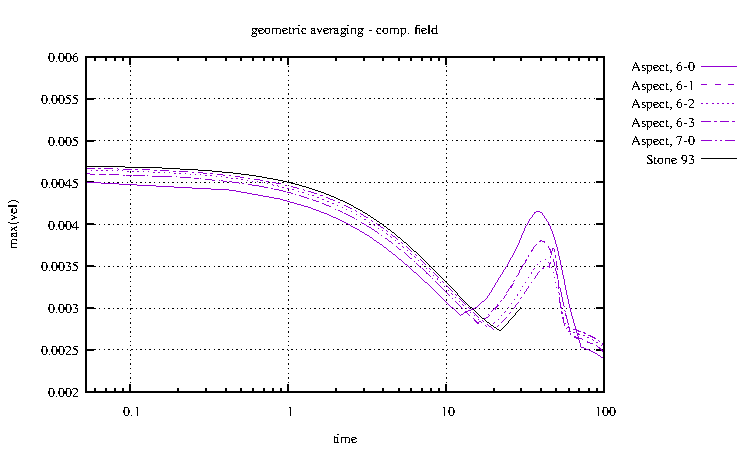
\includegraphics[width=5.7cm]{images/stokes_sphere_fs2D/max_vel_geom_comp}
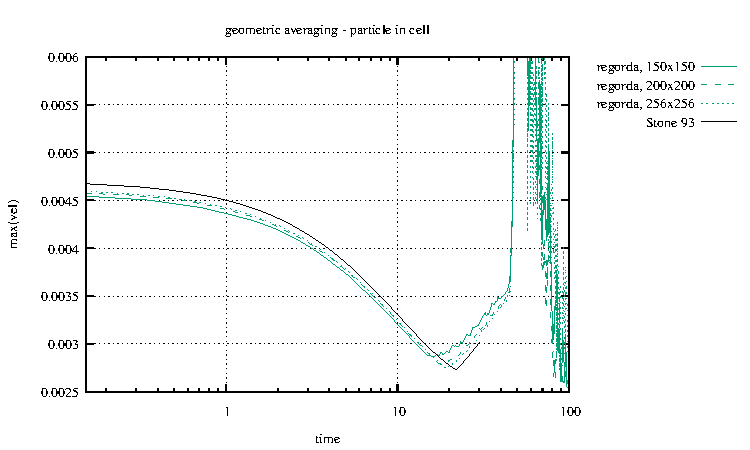
\includegraphics[width=5.7cm]{images/stokes_sphere_fs2D/max_vel_geom_pic}
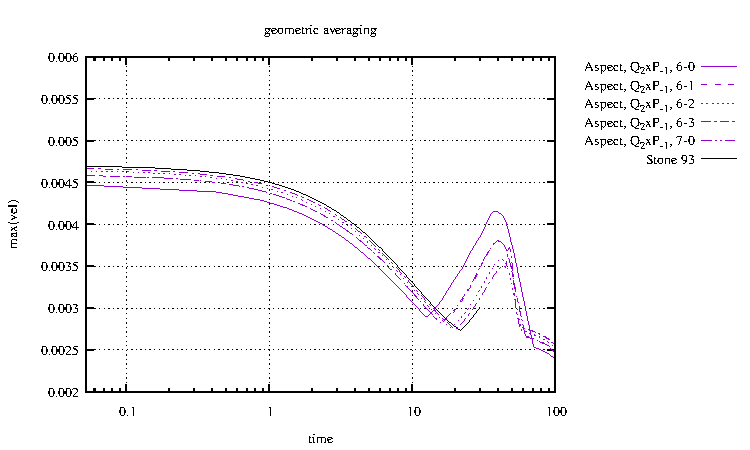
\includegraphics[width=5.7cm]{images/stokes_sphere_fs2D/max_vel_geom_add}\\
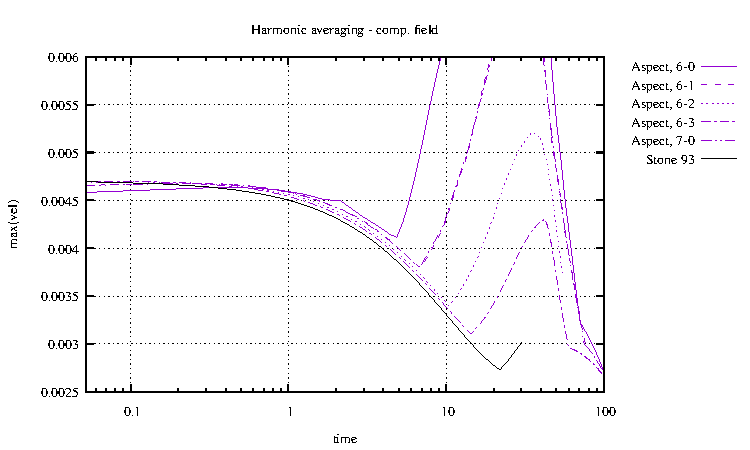
\includegraphics[width=5.7cm]{images/stokes_sphere_fs2D/max_vel_harm_comp}
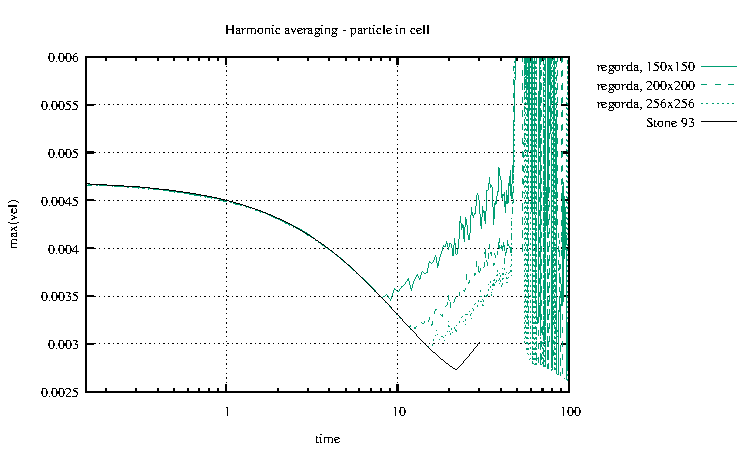
\includegraphics[width=5.7cm]{images/stokes_sphere_fs2D/max_vel_harm_pic}
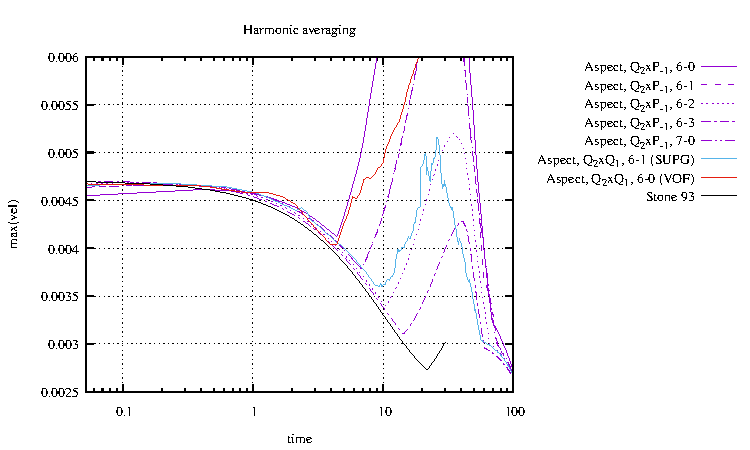
\includegraphics[width=5.7cm]{images/stokes_sphere_fs2D/max_vel_harm_add}
\end{center}


\paragraph{Compositions min/max}
\begin{center}
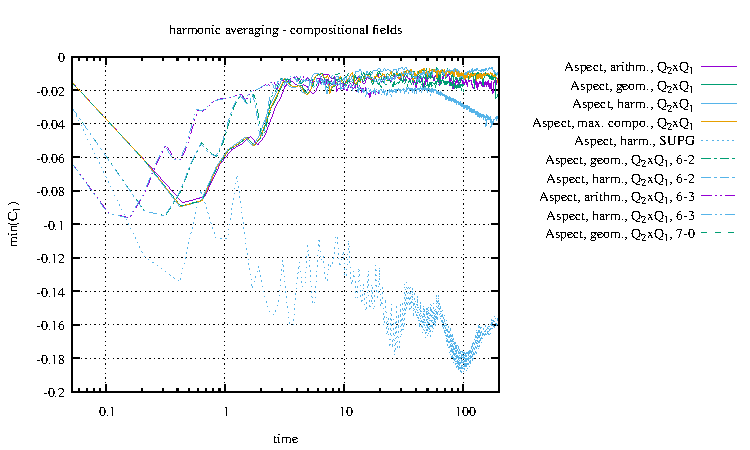
\includegraphics[width=7cm]{images/stokes_sphere_fs2D/C1_min}
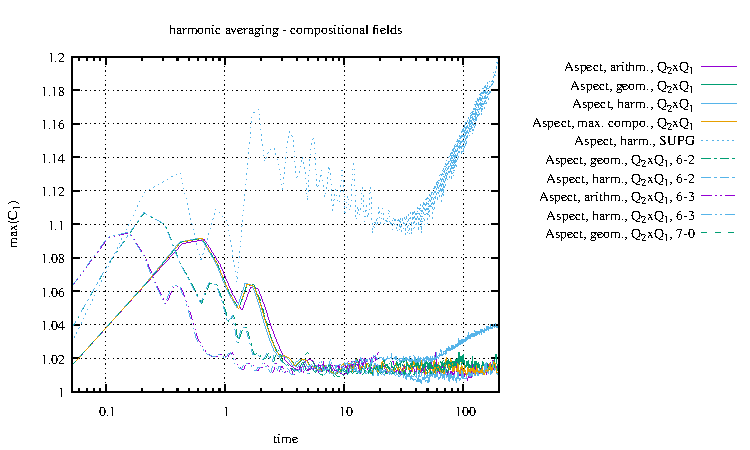
\includegraphics[width=7cm]{images/stokes_sphere_fs2D/C1_max}\\
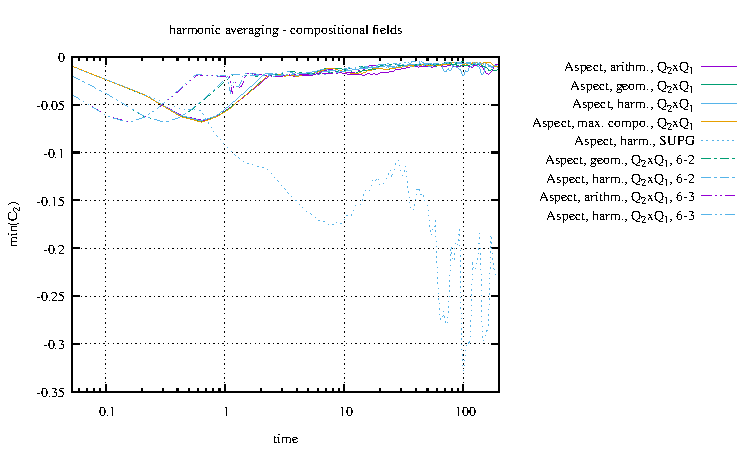
\includegraphics[width=7cm]{images/stokes_sphere_fs2D/C2_min}
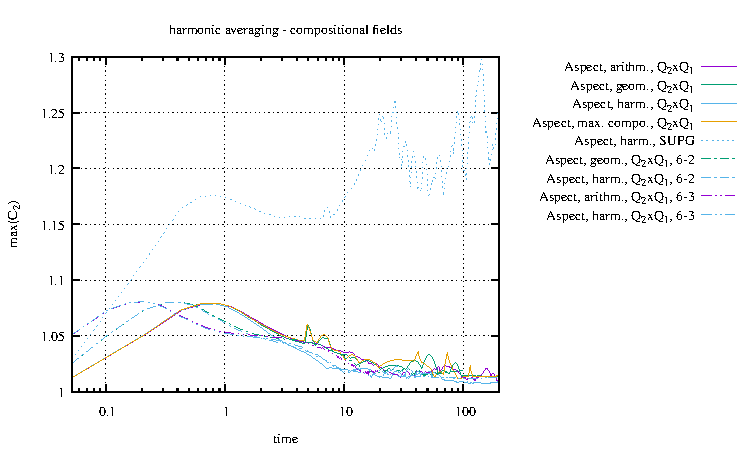
\includegraphics[width=7cm]{images/stokes_sphere_fs2D/C2_max}
\end{center}


\paragraph{Viscosity volume average}
\begin{center}
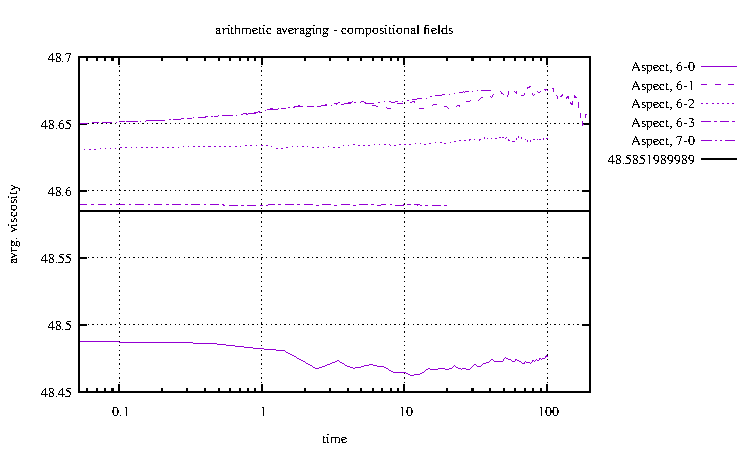
\includegraphics[width=5.7cm]{images/stokes_sphere_fs2D/avrg_viscosity_arithm_comp}
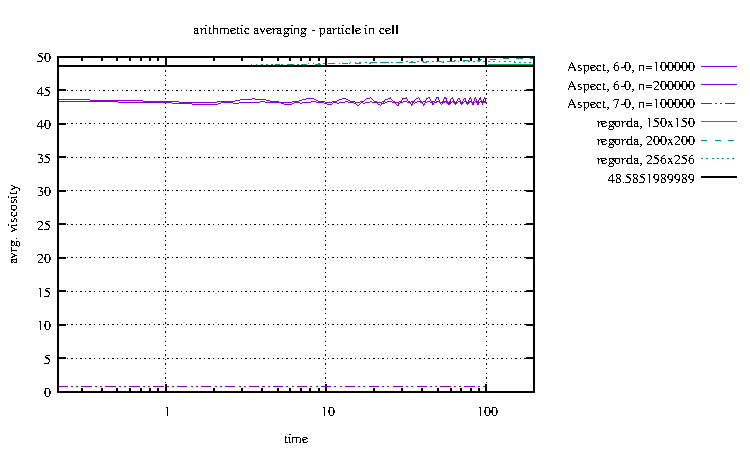
\includegraphics[width=5.7cm]{images/stokes_sphere_fs2D/avrg_viscosity_arithm_pic}\\
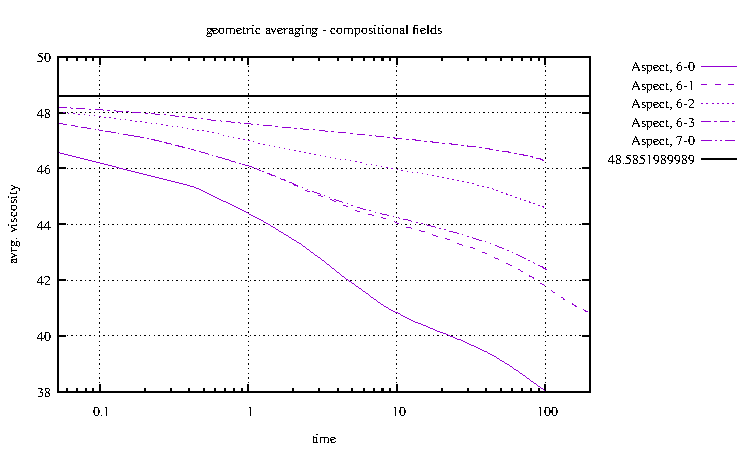
\includegraphics[width=5.7cm]{images/stokes_sphere_fs2D/avrg_viscosity_geom_comp}
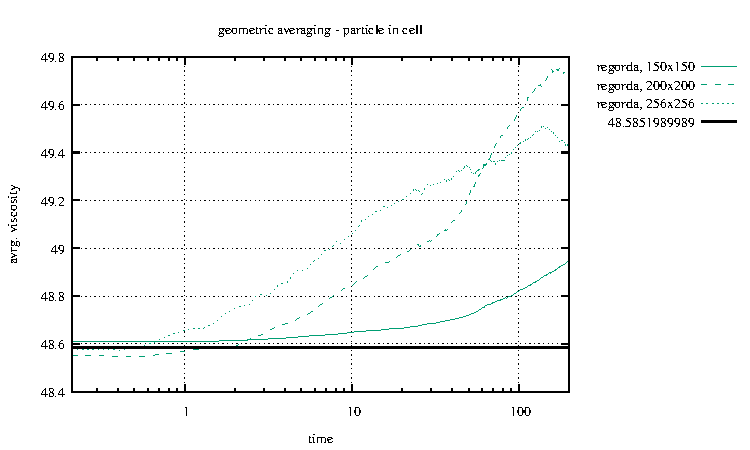
\includegraphics[width=5.7cm]{images/stokes_sphere_fs2D/avrg_viscosity_geom_pic}\\
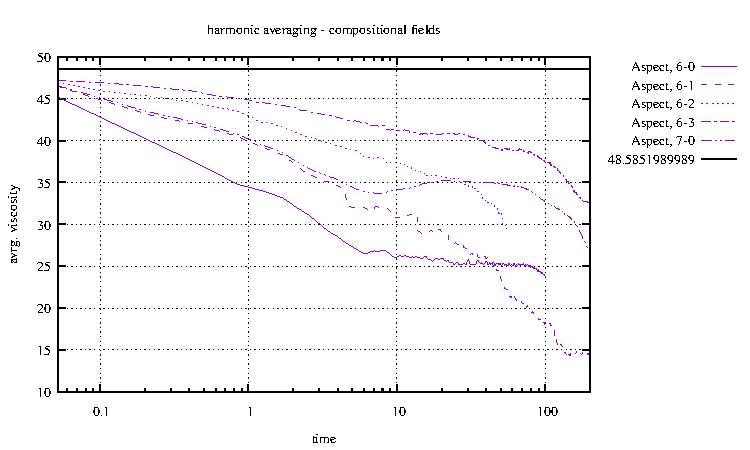
\includegraphics[width=5.7cm]{images/stokes_sphere_fs2D/avrg_viscosity_harm_comp}
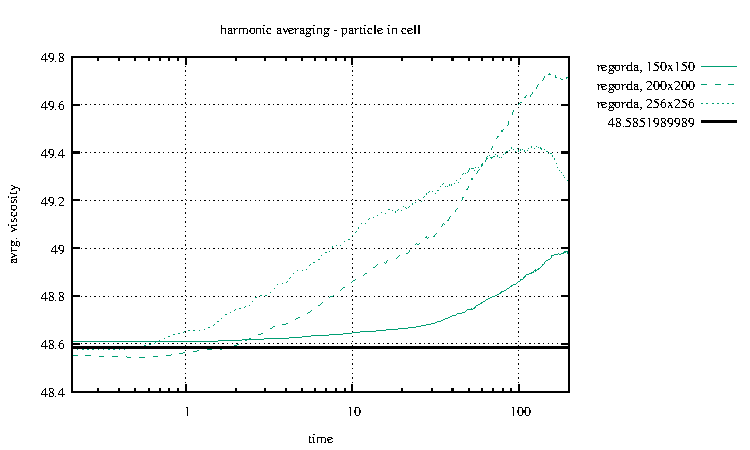
\includegraphics[width=5.7cm]{images/stokes_sphere_fs2D/avrg_viscosity_harm_pic}
\end{center}


\paragraph{Density volume average}
\begin{center}
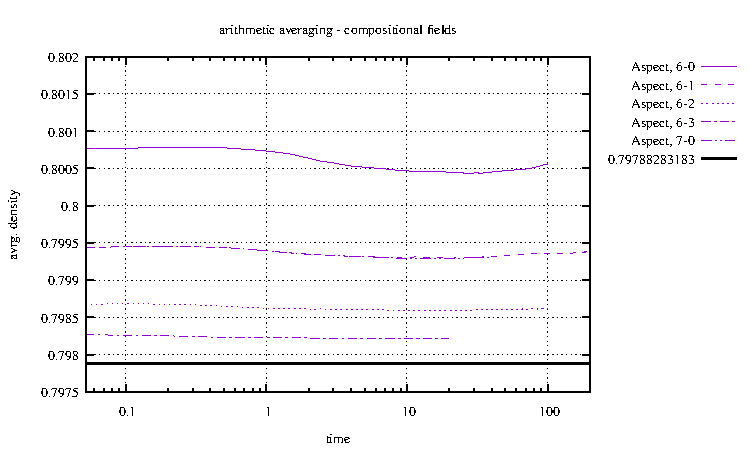
\includegraphics[width=5.7cm]{images/stokes_sphere_fs2D/avrg_density_arithm_comp}
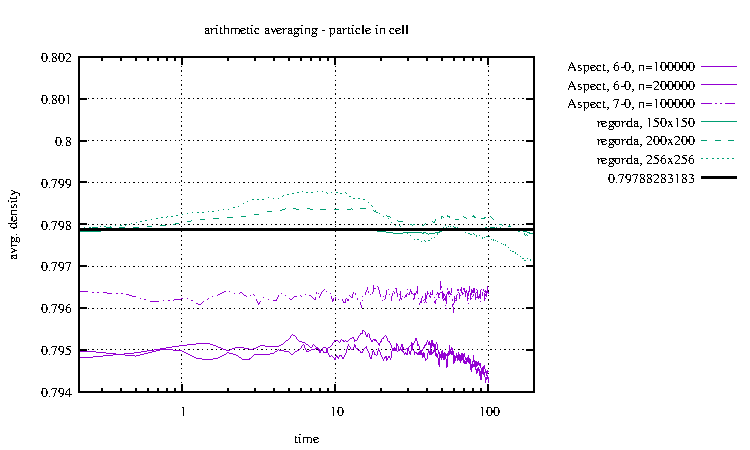
\includegraphics[width=5.7cm]{images/stokes_sphere_fs2D/avrg_density_arithm_pic}
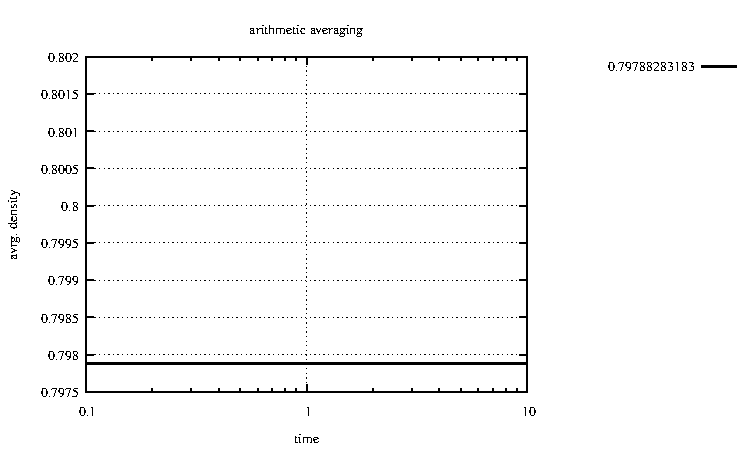
\includegraphics[width=5.7cm]{images/stokes_sphere_fs2D/avrg_density_arithm_add}\\
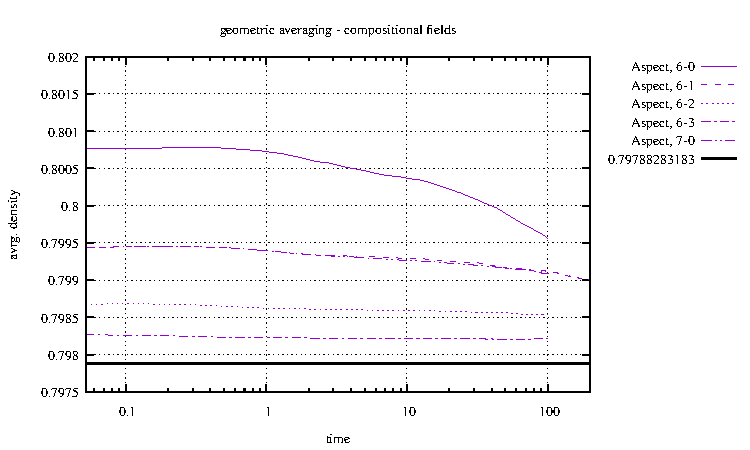
\includegraphics[width=5.7cm]{images/stokes_sphere_fs2D/avrg_density_geom_comp}
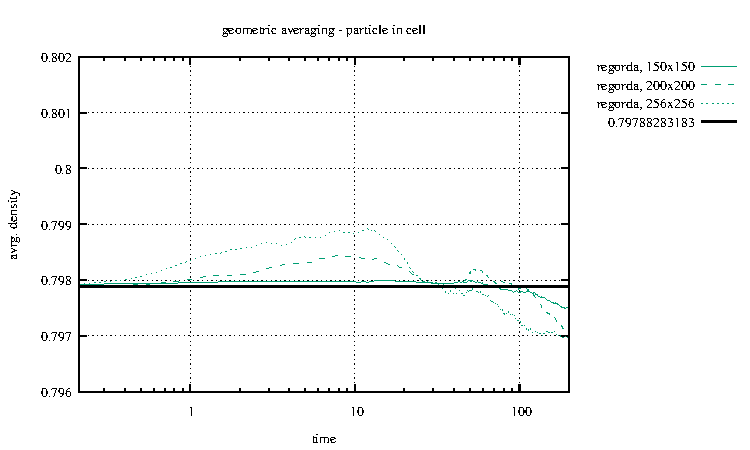
\includegraphics[width=5.7cm]{images/stokes_sphere_fs2D/avrg_density_geom_pic}
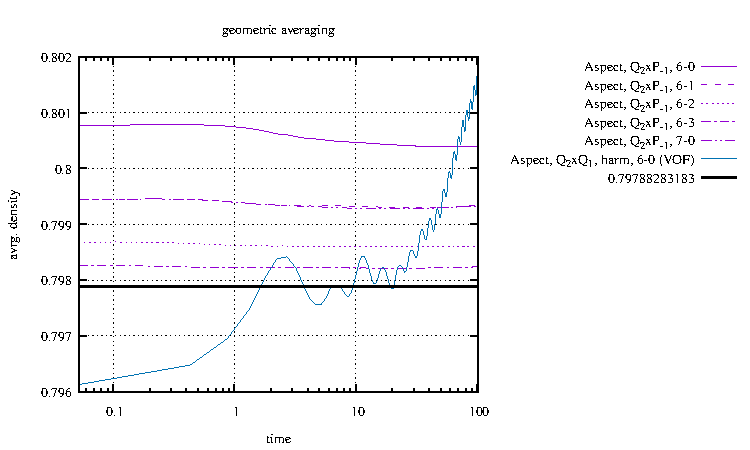
\includegraphics[width=5.7cm]{images/stokes_sphere_fs2D/avrg_density_geom_add}\\
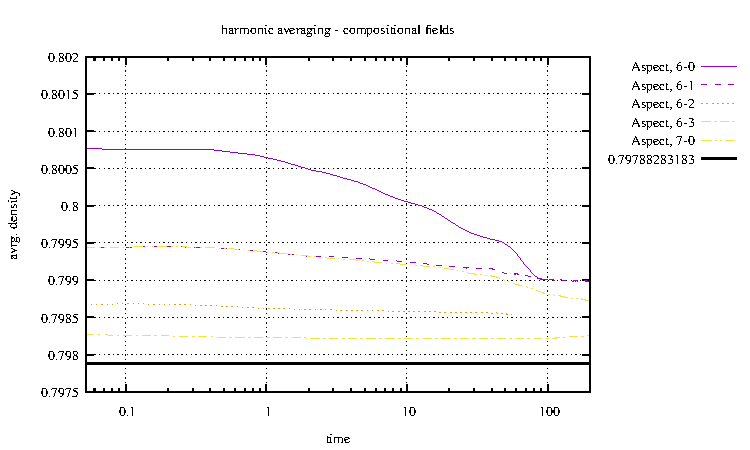
\includegraphics[width=5.7cm]{images/stokes_sphere_fs2D/avrg_density_harm_comp}
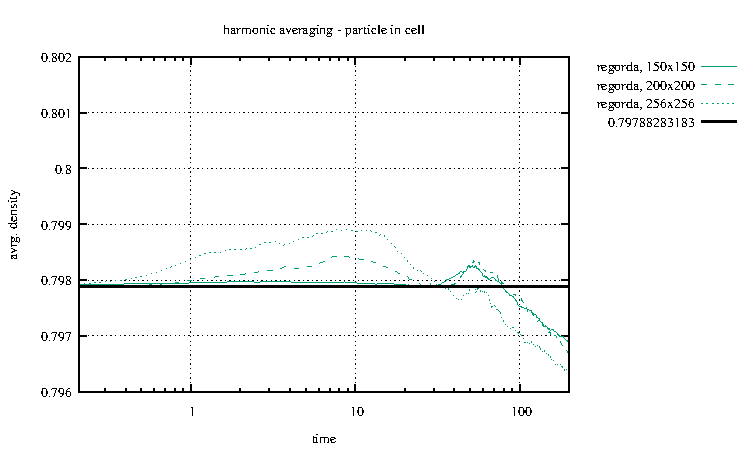
\includegraphics[width=5.7cm]{images/stokes_sphere_fs2D/avrg_density_harm_pic}
\includegraphics[width=5.7cm]{images/stokes_sphere_fs2D/avrg_density_harm_add}\\
\end{center}

\paragraph{Topography}
\begin{center}
\includegraphics[width=7cm]{images/stokes_sphere_fs2D/topography_min}
\includegraphics[width=7cm]{images/stokes_sphere_fs2D/topography_max}
\end{center}

\paragraph{Pressure measurements}
\begin{center}
\includegraphics[width=5.7cm]{images/stokes_sphere_fs2D/max_pressure_arithm_comp}
\includegraphics[width=5.7cm]{images/stokes_sphere_fs2D/max_pressure_arithm_pic}
\includegraphics[width=5.7cm]{images/stokes_sphere_fs2D/max_pressure_arithm_add}\\
\includegraphics[width=5.7cm]{images/stokes_sphere_fs2D/max_pressure_geom_comp}
\includegraphics[width=5.7cm]{images/stokes_sphere_fs2D/max_pressure_geom_pic}
\includegraphics[width=5.7cm]{images/stokes_sphere_fs2D/max_pressure_geom_add}\\
\includegraphics[width=5.7cm]{images/stokes_sphere_fs2D/max_pressure_harm_comp}
\includegraphics[width=5.7cm]{images/stokes_sphere_fs2D/max_pressure_harm_pic}
\includegraphics[width=5.7cm]{images/stokes_sphere_fs2D/max_pressure_harm_add}\\
\includegraphics[width=7cm]{images/stokes_sphere_fs2D/p_bottom}
\end{center}

\paragraph{Position of the sphere center}.
\begin{center}
\includegraphics[width=5cm]{images/stokes_sphere_fs2D/center_position_x_arithm_pic.pdf}
\includegraphics[width=5cm]{images/stokes_sphere_fs2D/center_position_x_geom_pic.pdf}
\includegraphics[width=5cm]{images/stokes_sphere_fs2D/center_position_x_harm_pic.pdf}\\
\includegraphics[width=5cm]{images/stokes_sphere_fs2D/center_position_y_arithm_pic.pdf}
\includegraphics[width=5cm]{images/stokes_sphere_fs2D/center_position_y_geom_pic.pdf}
\includegraphics[width=5cm]{images/stokes_sphere_fs2D/center_position_y_harm_pic.pdf}\\
\end{center}

\paragraph{Velocity of the sphere center}.
\begin{center}
\includegraphics[width=7.5cm]{images/stokes_sphere_fs2D/center_velocity_x.pdf}
\includegraphics[width=7.5cm]{images/stokes_sphere_fs2D/center_velocity_y.pdf}
\end{center}

\paragraph{Velocity at (0.5,0.6) location}.
\begin{center}
\includegraphics[width=5cm]{images/stokes_sphere_fs2D/point_u_arithm_comp}
\includegraphics[width=5cm]{images/stokes_sphere_fs2D/point_u_geom_comp}
\includegraphics[width=5cm]{images/stokes_sphere_fs2D/point_u_harm_comp}\\
\includegraphics[width=5cm]{images/stokes_sphere_fs2D/point_v_arithm_comp}
\includegraphics[width=5cm]{images/stokes_sphere_fs2D/point_v_geom_comp}
\includegraphics[width=5cm]{images/stokes_sphere_fs2D/point_v_harm_comp}\\
\includegraphics[width=5cm]{images/stokes_sphere_fs2D/point_v_arithm_pic}
\includegraphics[width=5cm]{images/stokes_sphere_fs2D/point_v_geom_pic}
\includegraphics[width=5cm]{images/stokes_sphere_fs2D/point_v_harm_pic}
\end{center}


\paragraph{Pressure at (0.5,0.6) location}.

\begin{center}
\includegraphics[width=5.7cm]{images/stokes_sphere_fs2D/point_p_arithm_comp}
\includegraphics[width=5.7cm]{images/stokes_sphere_fs2D/point_p_geom_comp}
\includegraphics[width=5.7cm]{images/stokes_sphere_fs2D/point_p_harm_comp}\\
\includegraphics[width=5.7cm]{images/stokes_sphere_fs2D/point_p_arithm_pic}
\includegraphics[width=5.7cm]{images/stokes_sphere_fs2D/point_p_geom_pic}
\includegraphics[width=5.7cm]{images/stokes_sphere_fs2D/point_p_harm_pic}
\end{center}

\paragraph{Material at (0.5,0.6) location}.

\begin{center}
\includegraphics[width=5.7cm]{images/stokes_sphere_fs2D/point_material_arithm_comp}
\includegraphics[width=5.7cm]{images/stokes_sphere_fs2D/point_material_geom_comp}
\includegraphics[width=5.7cm]{images/stokes_sphere_fs2D/point_material_harm_comp}\\
\includegraphics[width=5.7cm]{images/stokes_sphere_fs2D/point_material_arithm_pic}
\includegraphics[width=5.7cm]{images/stokes_sphere_fs2D/point_material_geom_pic}
\includegraphics[width=5.7cm]{images/stokes_sphere_fs2D/point_material_harm_pic}
\end{center}


\paragraph{Timestep and solver convergence}
\begin{center}
\includegraphics[width=7cm]{images/stokes_sphere_fs2D/dt_aspect}
\includegraphics[width=7cm]{images/stokes_sphere_fs2D/dt_pic}
\includegraphics[width=7cm]{images/stokes_sphere_fs2D/stokes_solver}
\end{center}

Stone 93 results seem to be most influenced by the resolution on the sphere and 
surface than the resolution in the fluid.
Some conclusions: arithmetic yields very high inner iteration counts. Discontinuous pressure
also better on that topic. Geometric averaging yields very good agreement for vrms.
Funny enough, geometric does not correspond to a physical arrangement of viscous dampers...
Arithm and harm do ultimately converge towards geom but at very high resolution.
Using no amr does not change things that much.  


\newpage
\begin{center}
\includegraphics[width=3.3cm]{images/stokes_sphere_fs2D/harm_6_1/grid0000}
\includegraphics[width=3.3cm]{images/stokes_sphere_fs2D/harm_6_1/grid0050}
\includegraphics[width=3.3cm]{images/stokes_sphere_fs2D/harm_6_1/grid0100}
\includegraphics[width=3.3cm]{images/stokes_sphere_fs2D/harm_6_1/grid0150}
\includegraphics[width=3.3cm]{images/stokes_sphere_fs2D/harm_6_1/grid0200}\\
\includegraphics[width=3.3cm]{images/stokes_sphere_fs2D/harm_6_1/eta0000}
\includegraphics[width=3.3cm]{images/stokes_sphere_fs2D/harm_6_1/eta0050}
\includegraphics[width=3.3cm]{images/stokes_sphere_fs2D/harm_6_1/eta0100}
\includegraphics[width=3.3cm]{images/stokes_sphere_fs2D/harm_6_1/eta0150}
\includegraphics[width=3.3cm]{images/stokes_sphere_fs2D/harm_6_1/eta0200}\\
\includegraphics[width=3.3cm]{images/stokes_sphere_fs2D/harm_6_1/vel0000}
\includegraphics[width=3.3cm]{images/stokes_sphere_fs2D/harm_6_1/vel0050}
\includegraphics[width=3.3cm]{images/stokes_sphere_fs2D/harm_6_1/vel0100}
\includegraphics[width=3.3cm]{images/stokes_sphere_fs2D/harm_6_1/vel0150}
\includegraphics[width=3.3cm]{images/stokes_sphere_fs2D/harm_6_1/vel0200}\\
\includegraphics[width=3.3cm]{images/stokes_sphere_fs2D/harm_6_1/p0000}
\includegraphics[width=3.3cm]{images/stokes_sphere_fs2D/harm_6_1/p0050}
\includegraphics[width=3.3cm]{images/stokes_sphere_fs2D/harm_6_1/p0100}
\includegraphics[width=3.3cm]{images/stokes_sphere_fs2D/harm_6_1/p0150}
\includegraphics[width=3.3cm]{images/stokes_sphere_fs2D/harm_6_1/p0200}\\
\includegraphics[width=3.3cm]{images/stokes_sphere_fs2D/harm_6_1/sr0000}
\includegraphics[width=3.3cm]{images/stokes_sphere_fs2D/harm_6_1/sr0050}
\includegraphics[width=3.3cm]{images/stokes_sphere_fs2D/harm_6_1/sr0100}
\includegraphics[width=3.3cm]{images/stokes_sphere_fs2D/harm_6_1/sr0150}
\includegraphics[width=3.3cm]{images/stokes_sphere_fs2D/harm_6_1/sr0200}\\
\includegraphics[width=3.3cm]{images/stokes_sphere_fs2D/harm_6_1/swarm_C1_0000}
\includegraphics[width=3.3cm]{images/stokes_sphere_fs2D/harm_6_1/swarm_C1_0050}
\includegraphics[width=3.3cm]{images/stokes_sphere_fs2D/harm_6_1/swarm_C1_0100}
\includegraphics[width=3.3cm]{images/stokes_sphere_fs2D/harm_6_1/swarm_C1_0150}
\includegraphics[width=3.3cm]{images/stokes_sphere_fs2D/harm_6_1/swarm_C1_0200}\\
\includegraphics[width=3.3cm]{images/stokes_sphere_fs2D/harm_6_1/swarm_C2_0000}
\includegraphics[width=3.3cm]{images/stokes_sphere_fs2D/harm_6_1/swarm_C2_0050}
\includegraphics[width=3.3cm]{images/stokes_sphere_fs2D/harm_6_1/swarm_C2_0100}
\includegraphics[width=3.3cm]{images/stokes_sphere_fs2D/harm_6_1/swarm_C2_0150}
\includegraphics[width=3.3cm]{images/stokes_sphere_fs2D/harm_6_1/swarm_C2_0200}\\
\includegraphics[width=3.3cm]{images/stokes_sphere_fs2D/harm_6_1/swarm_id0000}
\includegraphics[width=3.3cm]{images/stokes_sphere_fs2D/harm_6_1/swarm_id0050}
\includegraphics[width=3.3cm]{images/stokes_sphere_fs2D/harm_6_1/swarm_id0100}
\includegraphics[width=3.3cm]{images/stokes_sphere_fs2D/harm_6_1/swarm_id0150}
\includegraphics[width=3.3cm]{images/stokes_sphere_fs2D/harm_6_1/swarm_id0200}\\
{\captionfont \aspect results: fields and passive markers time evolution. 
Last row is the particle id, between 0 and 50000. 
System at times 0,50,100,150,200. Harmonic averaging.}
\end{center}



\newpage
\begin{center}
\includegraphics[width=4cm]{images/stokes_sphere_fs2D/aspects/C1_a}
\includegraphics[width=4cm]{images/stokes_sphere_fs2D/aspects/C1_g}
\includegraphics[width=4cm]{images/stokes_sphere_fs2D/aspects/C1_h}
\includegraphics[width=4cm]{images/stokes_sphere_fs2D/aspects/C1_m}\\
\includegraphics[width=4cm]{images/stokes_sphere_fs2D/aspects/C2_a}
\includegraphics[width=4cm]{images/stokes_sphere_fs2D/aspects/C2_g}
\includegraphics[width=4cm]{images/stokes_sphere_fs2D/aspects/C2_h}
\includegraphics[width=4cm]{images/stokes_sphere_fs2D/aspects/C2_m}\\
\includegraphics[width=4cm]{images/stokes_sphere_fs2D/aspects/sr_a}
\includegraphics[width=4cm]{images/stokes_sphere_fs2D/aspects/sr_g}
\includegraphics[width=4cm]{images/stokes_sphere_fs2D/aspects/sr_h}
\includegraphics[width=4cm]{images/stokes_sphere_fs2D/aspects/sr_m}\\
\includegraphics[width=4cm]{images/stokes_sphere_fs2D/aspects/eta_a}
\includegraphics[width=4cm]{images/stokes_sphere_fs2D/aspects/eta_g}
\includegraphics[width=4cm]{images/stokes_sphere_fs2D/aspects/eta_h}
\includegraphics[width=4cm]{images/stokes_sphere_fs2D/aspects/eta_m}\\
\includegraphics[width=4cm]{images/stokes_sphere_fs2D/aspects/rho_a}
\includegraphics[width=4cm]{images/stokes_sphere_fs2D/aspects/rho_g}
\includegraphics[width=4cm]{images/stokes_sphere_fs2D/aspects/rho_h}
\includegraphics[width=4cm]{images/stokes_sphere_fs2D/aspects/rho_m}\\
{\captionfont Obtained with Aspect. From left to right: Arithmetic, geometric, harmonic, maximum 
composition, all at $t=200$.}
\end{center}


\newpage

This is the \aspect input file for this benchmark:
 
\lstinputlisting[basicstyle=\tiny]{images/stokes_sphere_fs2D/sphere.prm}

